\newpage
\subsection{Поступление материалов}
\label{bp:MatInput}
%


\subsubsection{Поступление бумаги и картона}

Рулоны бумаги и картона принимаются кладовщиками на склад ролевой продукции. 
Поставщик высылает отвес-фактуру по электронной почте заранее. Документы получают в отделе закупок и передают на склад. Кладовщик по сырью заранее заполняет в системе 1С:УПП приходный ордер по номерам рулонов с указанием номенклатуры сырья, веса, метража, формата, номера рулона.

Кладовщик принимает машину с рулонами. Кладовщик принимает рулоны бумаги и картона по отвес-фактуре поставщика по номерам рулонов (рис. \ref{pic:d35}).  Кладовщик производит первичный осмотр качество рулонов, производит отбраковку в случае необходимости. Дефект рулона чаще всего связан с неправильной транспортировкой.  При необходимости кладовщик составляет акт дефектовки рулона.
При нарушении транспортировки  кладовщик составляет акт о повреждении и передает в ОТК. 
Рулон принимается на склад в любом случае.

При фактическом поступлении кладовщик из системы 1С:УПП печатает внутренние ярлыки на рулоны с номером рулона в виде QR-кода. Настроена печать на принтере этикеток по 2 штуки на рулон (рис. \ref{pic:d_Label}).
При поступлении машины кладовщик отмечает в системе 1С:УПП факт приемки в документе “Приходный ордер”. Кладовщик вес по факту не проверяет.

При отклонении от поставки Кладовщик составляет акт несоответствия по форме 033020 и передает акт в отдел снабжения.

Учет бумаги и картона выполняется в тоннах по документам. 
Водитель расставляет рулоны по рядам самостоятельно по маркам и форматам.
Кладовщик проверяет в конце дня расстановку рулонов, вручную ведет файл остатков по рулонам в файле Excel. 
Кладовщики посменно 24 часа по 12 часов.


Кладовщик передает документы по поступлению сырья в бухгалтерию.
При приемке материалов кладовщик создает акт в бухгалтерию по форме \ref{pic:d33}.

Бухгалтер дублирует документы поступления сырья в системе 1С:Бухгалтерия на основе приходных документов от поставщика.


% \subsubsection{Поступление рулонов бумаги и картона}

% Не производится.

% В форме к системе 1С 8 ''Управление торговлей'' ведутся данные по движению рулонов между площадками производство. В системе 1С 8 ''Управление торговлей'' данные по движению рулонов оперативны и достоверны.

% Диспетчер сообщает кладовщику о поступлении машины кладовщику. Кладовщик принимает машину с рулонами. Кладовщик принимает рулоны бумаги и картона по отвес-фактуре по номерам рулонов.  Кладовщик производит первичный осмотр качество рулонов, производит отбраковку в случае необходимости. Дефект рулона чаще всего связан с неправильной транспортировкой.  При необходимости кладовщик составляет акт дефектовки рулона. На каждую машину кладовщик составляет заключение по входному контролю качества сырья по  форме \ref{pic:pic_d49.1}.  На основании входного контроля старший кладовщик ведет журнал учета поврежденных рулонов (рис. \ref{pic:pic_d49.1}), которые будут списаны в производство в любом случае.  Входной контроль качества кладовщик передает в отдел технического контроля. Кладовщик передаёт накладную старшему кладовщику.   Комплект документов старший кладовщик передает в бухгалтерию, где заносят поступление сырья в систему 1С 8.3 ''Управление торговлей''. Остатки по сырью бумага и картон достоверные в системе 1С 8.3 ''Управление торговлей''. При этом кладовщик всё равно создает вручную отчет по остаткам (рис. \ref{pic:pic_d25}). Кладовщик каждый день пересчитывает остатки по рулонам. Расхождение могут быть один раз в месяц.


\subsubsection{Поступление прочих материалов}

Поступление прочих материалов от поставщика по УПД кладовщик выполняет в системе 1С:УПП. Кладовщик создает документ “Приходный ордер”.

Краску на производство принимает кладовщик. Краска приходит на производство и хранится в ведрах по 20 кг. 
Учетом краски занимается участок ОТК. 





% На производстве краску техник УВФ замешивает по рецептуре из программы IMS (рис. \ref{pic:f16}, \ref{pic:f17}) из основы и пигментов. 

% При поступлении краски и основы на предприятие техники УВФ создают приход в программе СБИС. 

% При получении плана на производство на смену техники УВФ замешивают необходимую краску согласно понтону в ТК. Объем краски определяют из опыта, расчета краски не выявлено. 
% После приготовления краски распечатывают и приклеивают ярлык на ведро с указанием номера понтона и веса краски (рис. \ref{pic:f20}).

% Краска хранится на УВФ (рис. \ref{pic:f18}, \ref{pic:f19}).


% Вспом материалы принимает техник по учету в системе СБИС (остальные материалы, спецодежда, канцелярские товары и проч.)




% Поступившую краску принимает мастер и  ставит в специально отведенное место для хранения (рис. \ref{pic:a12}). 

% Вспомогательные материалы (клей, лента и пр) кладовщик принимает на склад согласно документам поступления. 
% Полученные накладные кладовщик передает в бухгалтерию, где бухгалтер оприходует материалы в системе 1С:УНФ документом «Поступление ТМЦ». 

\begin{figure}
\begin{center}
  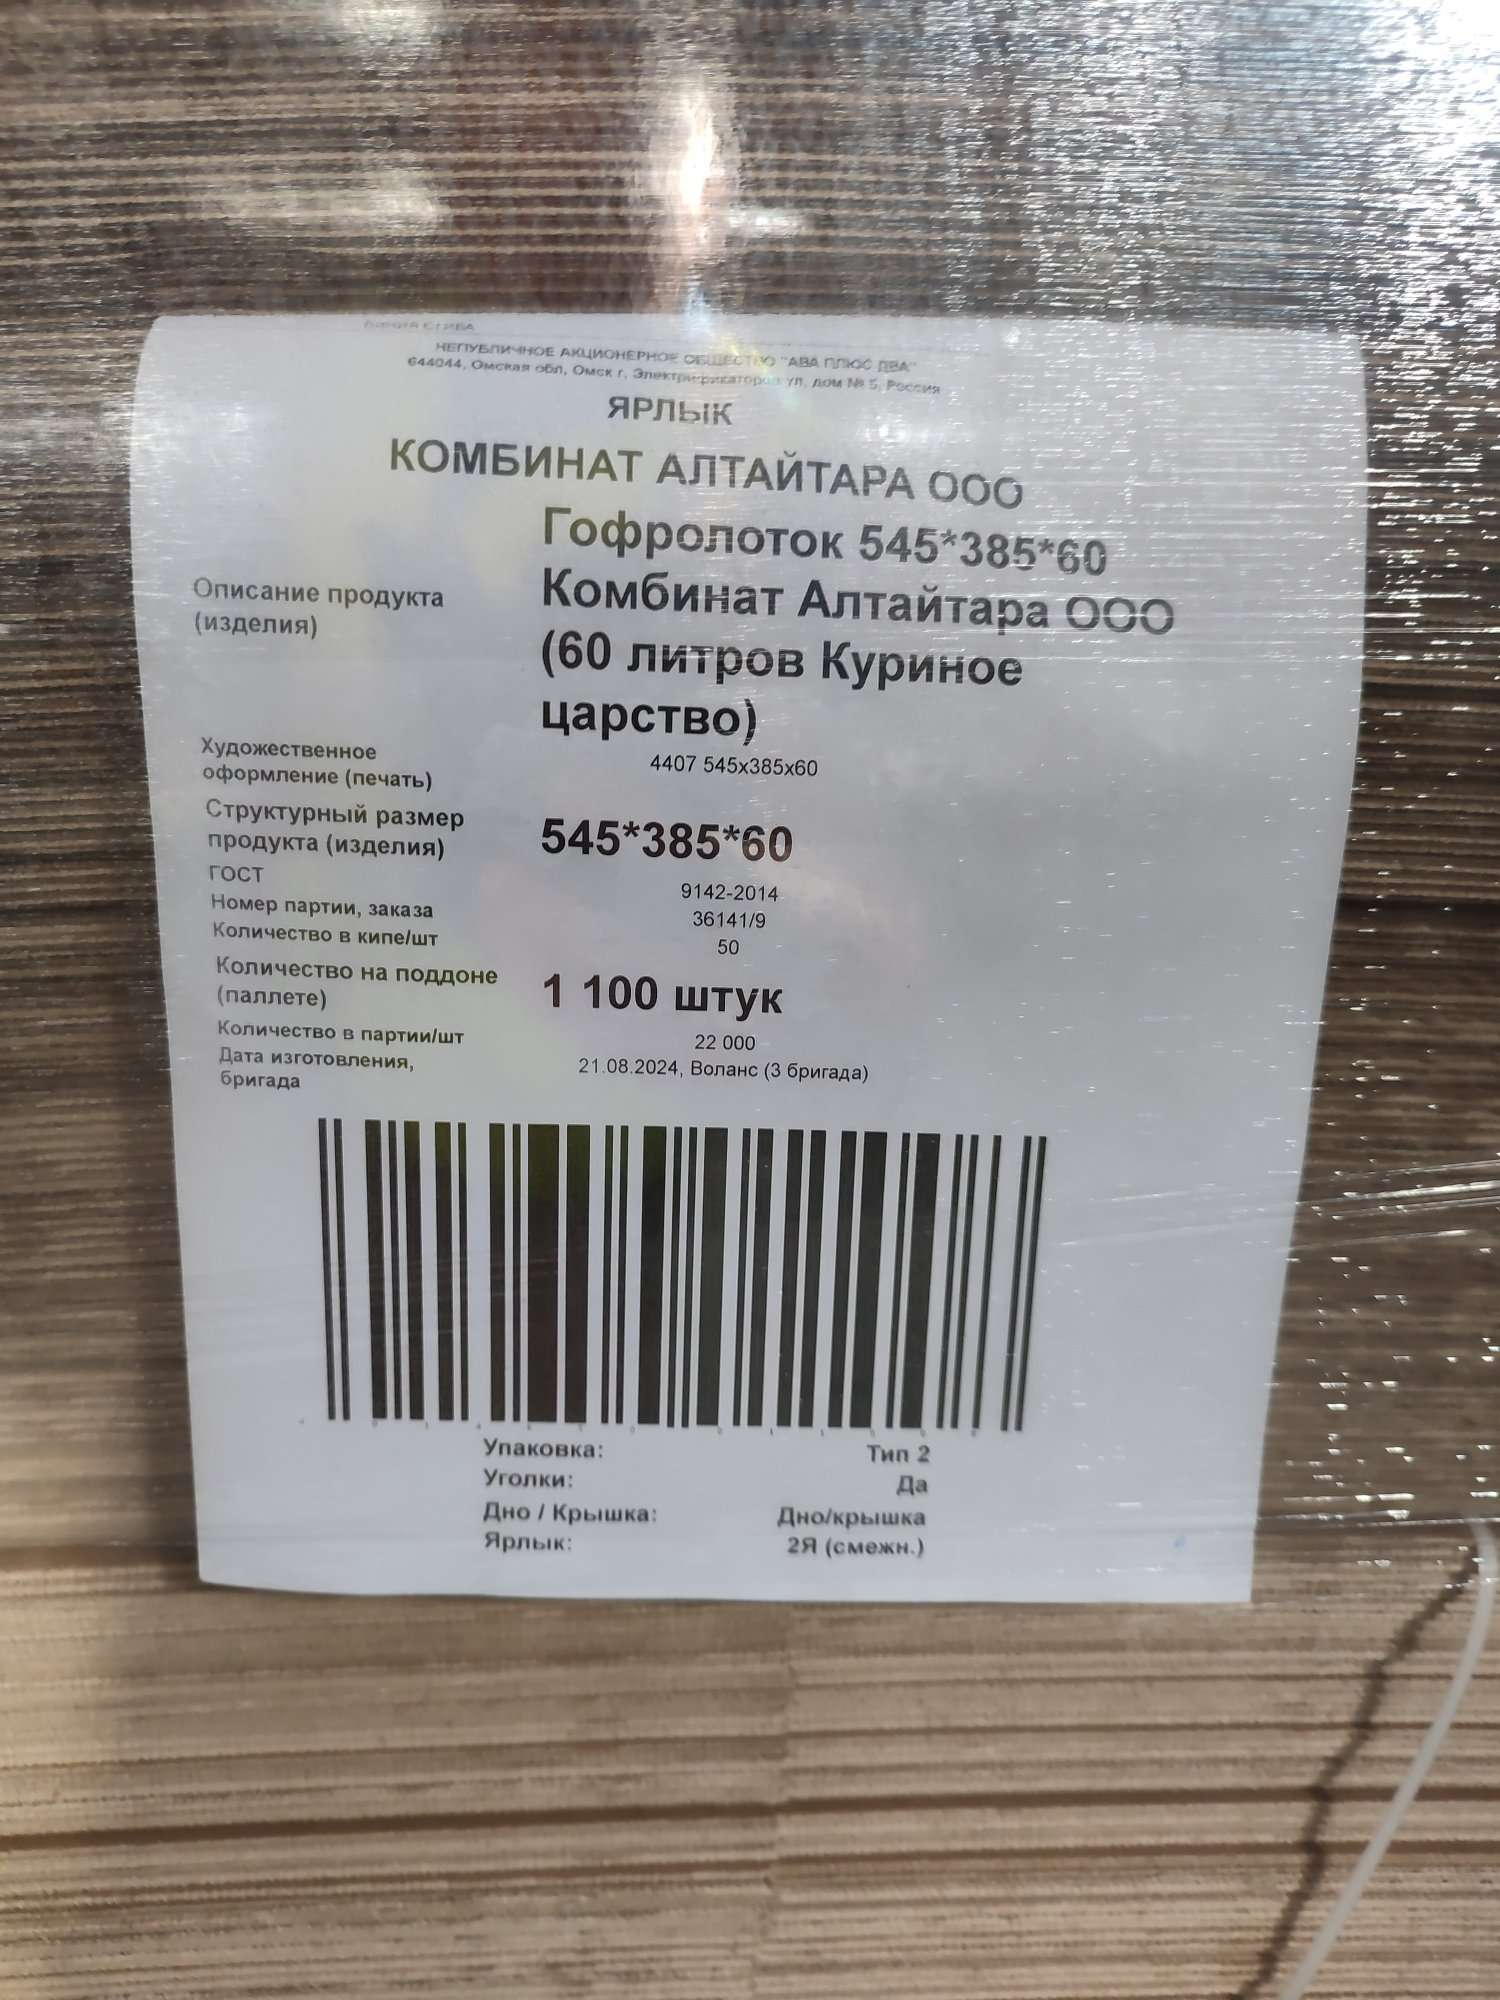
\includegraphics[height=0.94\textheight, width=\textwidth, keepaspectratio]{Pics/d_Label.JPEG}
\end{center}
  \caption{Внутренняя бирка со штрих-кодом на рулон}
  \label{pic:d_Label}
\end{figure}

% \begin{figure}
% \begin{center}
%   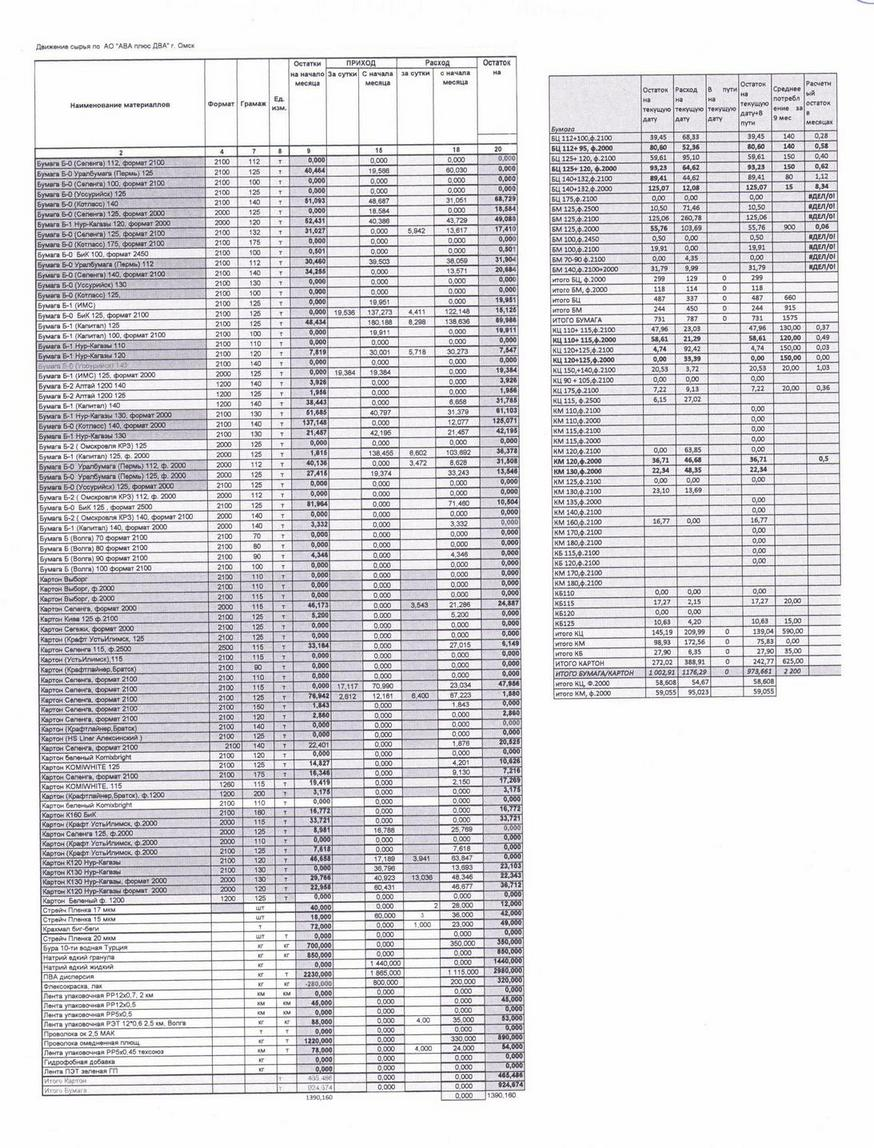
\includegraphics[height=0.94\textheight, width=\textwidth, keepaspectratio]{Pics/d35.jpg}
% \end{center}
%   \caption{Отвес-фактура по рулонам бумаги и картона}
%   \label{pic:d35}
% \end{figure}

% \begin{figure}
% \begin{center}
%   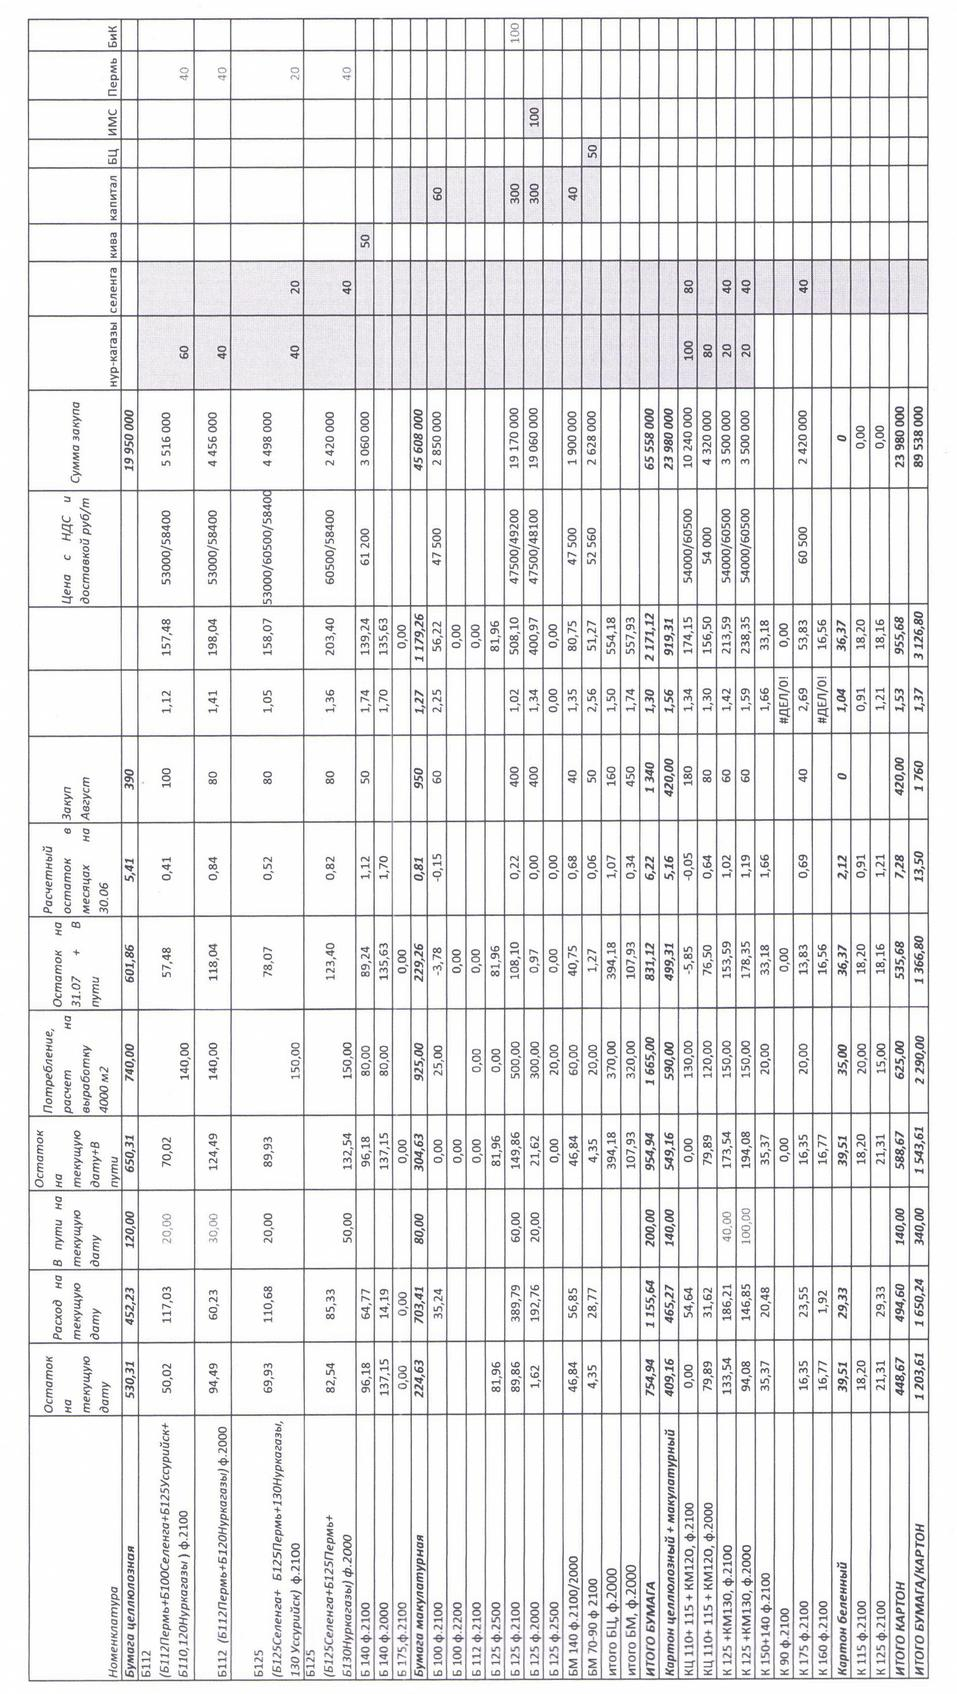
\includegraphics[height=0.8\textheight, width=\textwidth, keepaspectratio]{Pics/d37.jpg}
% \end{center}
%   \caption{Акт о повреждении продукции}
%   \label{pic:d37}
% \end{figure}


% \begin{figure}
% \begin{center}
%   \includegraphics[height=0.94\textheight, width=0.94\textwidth, keepaspectratio]{Pics/f20.jpg}
% \end{center}
%   \caption{Ярлык на краску}
%   \label{pic:f20}
% \end{figure}



% \begin{figure}
% \begin{center}
%   \includegraphics[height=0.94\textheight, width=0.94\textwidth, keepaspectratio]{Pics/a9.jpg}
% \end{center}
%   \caption{Отчет по поступлению краски}
%   \label{pic:a9}
% \end{figure}


\clearpage
\ifx \notincludehead\undefined
\normalsize
\end{document}
\fi